\documentclass[12pt]{article}
\title{EE351K Homework 6}
\author{Hershal Bhave (hb6279)}
\date{Due October 16, 2014}

\usepackage{multicol}
\usepackage[in]{fullpage}
\usepackage{xcolor}
\usepackage{rotating}
\usepackage{mathtools}
\usepackage{amssymb}
\usepackage{cleveref}
\usepackage{graphics}
\usepackage{caption}
\usepackage{wrapfig}
\usepackage{subcaption}
\usepackage[nosolutionfiles]{answers}
\usepackage[acronym]{glossaries}

\newenvironment{Ex}{\textbf{Problem}\vspace{.75em}\\}{}
\Newassociation{solution}{Soln}{Answers}
\pagebreak[3]
\newcommand{\Opentesthook}[2]{\Writetofile{#1}{\protect\section{#1: #2}}}
\renewcommand{\Solnlabel}[1]{\textbf{Solution}\quad}

\newcommand{\dd}[1]{\:\mathrm{d}{#1}}
\newcommand{\ddt}[1]{\frac{\dd{}}{\dd{#1}}}
\newcommand{\dddt}[1]{\frac{\dd{}^2}{\dd{#1}^2}}

\begin{document}
\maketitle
\begin{enumerate}
\item
  \begin{Ex}
    Random Variables $X$ and $Y$ are described by the joint PDF
    \begin{equation}
      \label{eq:1-question}
      f_{X,Y}(x,y) = \left\{
        \begin{aligned}
          & ax &&\quad 2\le x\le 4,\quad 0\le y \le x \\
          & 0 &&\quad \text{otherwise} \\
        \end{aligned}\right.
    \end{equation}
    \begin{enumerate}
    \item Evaluate the constant $a$.
    \item Determine the marginal PDF $f_Y(y)$.
    \item Determine the expected value for $\frac{1}{X}$ given that $Y=3$.
    \end{enumerate}
    \begin{solution} \hfill
      \begin{enumerate}
      \item The constant $a$ can be determined by integrating across
        the area which $f_{X,Y}$ is defined and setting it equal to 1.
        \begin{equation}
          \label{eq:1a-presol}
          \begin{aligned}
            1 &= \int_0^x \int_2^4 ax \dd{x} \dd{y} \\
          \end{aligned}
        \end{equation}
        We can reverse the integrals to get an exact result
        \begin{equation}
          \label{eq:1a-sol}
          \begin{aligned}
            1 &= \int_2^4 \int_0^x ax \dd{y} \dd{x} \\
            &= a \int_2^4 x \int_0^x 1 \dd{y} \dd{x} \\
            &= a \int_2^4 x \; [y]_0^x \dd{x} \\
            &= a \int_2^4 x^2 \dd{x} \\
            &= a \left[\frac{x^3}{3}\right]_2^4 \dd{x} \\
            &= a \left(\frac{64}{3} - \frac{8}{3}\right) \\
            \implies a&=\frac{3}{56} \\
          \end{aligned}
        \end{equation}
      \item Marginals can be computed by the following
        \begin{equation}
          \label{eq:1b-marginal-def}
          f_Y(y) = \int_{-\infty}^{\infty} f_{X,Y}(x,y) \dd{x}
        \end{equation}
        So we can insert our PDF into this equation to obtain the
        proper marginal.
        \begin{equation}
          \label{eq:1b-sol}
          \begin{aligned}
            f_Y(y) &= \int_{y}^{4} ax \dd{x} \\
            &= a \int_{y}^{4} x \dd{x} \\
            &= a \left[\frac{x^2}{2}\right]_y^4 \\
            \implies f_Y(y) &= a \left(8 - \frac{y^2}{2}\right) \\
          \end{aligned}
        \end{equation}
        Which means that the marginal from 2 to 4 is $f_Y(y) =
        \frac{9}{28}$.
      \item The Expected Value in this situation can be calculated
        by
        \begin{equation}
          \label{eq:1c-expected-value}
          E[g(X)|Y=y] = \int_{-\infty}^{\infty} g(x)f_{X|Y}(x|y) \dd{x}
        \end{equation}
        where
        \begin{equation}
          \label{eq:1c-conditional-value}
          f_{X|Y}(x|y) = \frac{f_{X,y}(x,y)}{f_Y(y)}
        \end{equation}
        So the equation we need turns out to be
        \begin{equation}
          \label{eq:1c-sol}
          \begin{aligned}
            E\left[\frac{1}{X}|Y=3\right] &= \int_{3}^{4}
            \frac{1}{x} \frac{f_{X,Y}(x,y)}{f_Y(y)} \dd{x} \\
            &= \int_{3}^{4} \frac{1}{x} \frac{ax}{a\left(8 -
                \frac{y^2}{2}\right)} \dd{x} \\
            &= \int_{3}^{4} \frac{1}{x} \frac{x}{8 - \frac{3^2}{2}}
            \dd{x} \\
            &= \int_{3}^{4} \frac{1}{x} \frac{x}{\frac{7}{2}} \dd{x} \\
            &= \int_{3}^{4} \frac{1}{x} \frac{2x}{7} \dd{x} \\
            &= \int_{3}^{4} \frac{2}{7} \dd{x} \\
            \implies E\left[\frac{1}{X}|Y=3\right] &= \frac{2}{7} \\
          \end{aligned}
        \end{equation}
      \end{enumerate}
    \end{solution}
  \end{Ex}
\item
  \begin{Ex}
    Suppose $X$ and $Y$ are described by the joint PDF
    \begin{equation}
      \label{eq:2-question}
      f_{X,Y}(x,y) = \left\{
        \begin{aligned}
          &5x^2/2 &&\quad -1 \le x \le 1, \quad 0\le y \le x^2 \\
          &0 &&\quad \text{otherwise} \\
        \end{aligned} \right.
    \end{equation}
    Let $A$ be the event that $\{Y\le 1/3\}$
    \begin{enumerate}
    \item What is the conditional joint density $f_{X,Y|A}(x,y)$?
    \item What are $f_{Y|A}(y)$ and $f_{X|A}(x)$?
    \item What are $E[Y|A]$ and $E[X|A]$?
    \end{enumerate}
    \begin{solution} \hfill
      \begin{enumerate}
      \item The way to obtain the conditional joint density is through
        the formula
        \begin{equation}
          \label{eq:2a-conditional-joint-density}
          f_{X,Y|A} = \left\{
            \begin{aligned}
              & \frac{f_{X,Y}(x,y)}{P(A)} &&\quad(x,y) \in A \\
              & 0 &&\quad\text{otherwise} \\
            \end{aligned} \right.
        \end{equation}
        In order to use that though, we must obtain the CDF for
        $P(A)$, where
        \begin{equation}
          \label{eq:2a-cdf-def}
          P(A) = P(Y \le y) = \int_{-\infty}^{y} f_{Y}(y) \dd{y}
        \end{equation}
        We must obtain the marginal $f_Y(y)$ in order to use
        \cref{eq:2a-conditional-joint-density}. We will do that now

        Now we can plug that into \cref{eq:2a-cdf-def}:
        \begin{equation}
          \label{eq:2a-marginal-b}
          f_Y(y) = \int_{B} f_{X,Y}(x,y) \dd{x}
        \end{equation}
        We determine the bounds $B$ before we can continue with the
        integration. Since $y$ is bounded by $0\le y \le x^2$, we can
        write
        \begin{equation}
          \label{eq:2a-y-bounds}
          \begin{aligned}
            & y \le x^2 \\
            & x^2 \ge y \\
            \implies & x \ge \sqrt{y},\; x \le -\sqrt{y} \\
          \end{aligned}
        \end{equation}
        But since $x$ is also already bounded by $-1 \le x \le 1$, the
        new bounds for $B$ are
        \begin{equation}
          \label{eq:2a-new-y-bounds}
          B \in \left\{-1\le x\le-\sqrt{\frac{1}{3}},\;
            \sqrt{\frac{1}{3}}\le x\le1\right\}
        \end{equation}
        The integral in \cref{eq:2a-marginal-b} then turns into
        \begin{equation}
          \label{eq:2a-marginal}
          \begin{aligned}
            f_Y(y) &= \int_{-1}^{-\sqrt{y}} f_{X,Y}(x,y)
            \dd{x} + \int_{\sqrt{y}}^{1} f_{X,Y}(x,y)
            \dd{x}\\
            \implies f_Y(y) &= \frac{5}{3}-\frac{5y^{3/2}}{3} \\
          \end{aligned}
        \end{equation}
        Now that we have the the marginal PDF, we can finally obtain
        the CDF for $P(A)$ using the equation given in \cref{eq:2a-cdf-def}
        \begin{equation}
          \label{eq:2a-cdf-plugged}
          \begin{aligned}
            P\left(Y \le \frac{1}{3}\right) &= \int_{0}^{1/3}
            f_{Y}(y) \dd{y} \\
            &= \int_{0}^{1/3} \frac{5}{3}-\frac{5y^{3/2}}{3}
            \dd{y} \\
            \implies P\left(Y \le \frac{1}{3}\right) &=
            \frac{45-2\sqrt{3}}{81} \\
          \end{aligned}
        \end{equation}
        So now we can obtain the conditional joint density
        \begin{equation}
          \label{eq:2a-conditional-joint-density-plugged}
          \begin{aligned}
            f_{X,Y|A}(x,y) &= \frac{f_{X,Y}(x,y)}{P(Y \le 1/3)} \\
            &= \frac{\frac{5x^2}{2}}{\frac{45-2\sqrt{3}}{81}} \\
            f_{X,Y|A}(x,y) &= \frac{405x^2}{2(45-2\sqrt{3})} \\
          \end{aligned}
        \end{equation}
        Or, more precisely
        \begin{equation}
          \label{eq:2a-sol}
          \implies f_{X,Y|A}(x,y) = \left\{
            \begin{aligned}
              & \frac{405x^2}{2(45-2\sqrt{3})} &&\quad (x,y) \in A \\
              & 0 &&\quad\text{otherwise} \\
            \end{aligned}\right.
        \end{equation}
      \item Now we must find the marginals $f_Y(y)$ and $f_X(x)$
        conditional on $A$.
        \begin{equation}
          \label{eq:2b-fy-def}
          f_{Y|A}(y) = \left\{
            \begin{aligned}
              & \frac{f_Y(y)}{P(A)} &&\quad y \in A \\
              & 0 &&\quad\text{otherwise} \\
            \end{aligned}\right.
        \end{equation}
        Since we already have the marginal $f_Y(y)$ from
        \cref{eq:2a-marginal} and $P(A)$ from
        \cref{eq:2a-cdf-plugged}, we can simply use those values here
        \begin{equation}
          \label{eq:2b-fy-presol}
          f_{Y|A}(y) = \left\{
            \begin{aligned}
              & \frac{\frac{5-5y^{3/2}}{3}}{\frac{45-2\sqrt{3}}{81}}
              &&\quad y \in A \\
              & 0 &&\quad\text{otherwise} \\
            \end{aligned}\right.
        \end{equation}
        Which, simplified, turns out to be
        \begin{equation}
          \label{eq:2b-fy-sol}
          \implies f_{Y|A}(y) = \left\{
            \begin{aligned}
              & \frac{81 \left(\frac{5}{3}-\frac{5
                    y^{3/2}}{3}\right)}{45-2 \sqrt{3}} &&\quad (x,y)
              \in A \\
              & 0 &&\quad\text{otherwise} \\
            \end{aligned}\right.
        \end{equation}
        Obtaining the marginal $f_X(x)$ is a similar process as
        \cref{eq:2a-marginal-b}, replacing $y$ with $x$.
        \begin{equation}
          \label{eq:2b-fx-prepresol}
          f_X(x) = \left\{
            \begin{aligned}
              & \int_{B} f_{Y,X}(y,x) \dd{y} &&\quad x \in A \\
              & 0 &&\quad\text{otherwise} \\
            \end{aligned} \right.
        \end{equation}
        Where $B$ in our case is simply $0 \le x \le 1/3$.
        \begin{equation}
          \label{eq:2b-fx-presol}
          \begin{aligned}
            f_X(x) &= \int_{B} f_{Y,X}(y,x) \dd{y} \\
            &= \int_0^{1/3} \frac{5x^2}{2} \dd{y} \\
            &= \frac{5x^2}{2} \int_0^{1/3} 1 \dd{y} \\
            \implies f_X(x) &= \frac{5x^2}{6} \\
          \end{aligned}
      \end{equation}
      Now we can use $P(A)$ obtained from \cref{eq:2a-cdf-plugged}
      to obtain $f_{X|A}(x)$
      \begin{equation}
        \label{eq:2b-fx-sol-raw}
        f_{X|A}(x) = \left\{
          \begin{aligned}
            & \frac{\frac{5x^2}{6}}{\frac{45-2\sqrt{3}}{81}} &&\quad
            x\in A \\
            & 0 && \quad\text{otherwise} \\
          \end{aligned} \right.
      \end{equation}
      Or alternatively
      \begin{equation}
        \label{eq:2b-fx-sol}
        \implies f_{X|A}(x) = \left\{
          \begin{aligned}
            & \frac{135 x^2}{2 \left(45-2 \sqrt{3}\right)} &&\quad
            x\in A \\
            & 0 && \quad\text{otherwise} \\
          \end{aligned} \right.
      \end{equation}
    \item The expected values for $X$ and $Y$ given $A$ can be
      computed by using \cref{eq:2b-fx-sol} and \cref{eq:2b-fy-sol},
      respectively. The range for the expected values for $E[X|A]$ is
      $B\in \left\{-1\le x\le-\sqrt{\frac{1}{3}},\;
        \sqrt{\frac{1}{3}}\le x\le1\right\}$.
      \begin{equation}
        \label{eq:2c-expected-x}
        \begin{aligned}
          E[X|A] &= \int_B x\;f_{X|A}(x) \dd{x} \\
          &= 2 \int_{\sqrt{\frac{1}{3}}}^{1} \frac{135 x^3}{2 \left(45-2 \sqrt{3}\right)} \dd{x} \\
          \implies E[X|A] &= \frac{30}{45-2 \sqrt{3}} \\
        \end{aligned}
      \end{equation}
      The range for the expected values for $E[Y|A]$ is $B \in \{0 \le
      y \le 1/3\}$
      \begin{equation}
        \label{eq:2c-expected-y}
        \begin{aligned}
          E[Y|A] &= \int_B y\;f_{Y|A}(y) \dd{y} \\
          &= \int_0^{1/3} \frac{81 y \left(\frac{5}{3}-\frac{5
                y^{3/2}}{3}\right)}{45-2 \sqrt{3}} \dd{y} \\
          \implies E[Y|A] &= -\frac{5 \left(18
              \sqrt{3}-937\right)}{28182} \\
        \end{aligned}
      \end{equation}
    \end{enumerate}
  \end{solution}
\end{Ex}
\item
  \begin{Ex}
    Suppose $X$ has PDF:
    \begin{equation}
      \label{eq:3-question}
      f_X(x) = \left\{
        \begin{aligned}
          &\frac{x}{2} &&\quad 0\le x\le 2 \\
          &0 &&\quad \text{otherwise} \\
        \end{aligned}\right.
    \end{equation}
    Where $X$ denotes the length of a stick. Now suppose the stick is
    randomly broken and let $Y$ denote the length of the remaining
    stick.
    \begin{enumerate}
    \item Find the joint PDF of $Y$ and $X$.
    \item Find the marginal PDF of $Y$.
    \item Find $E[Y]$.
    \end{enumerate}
    \begin{solution} \hfill
      \begin{enumerate}
      \item $Y$ is conditional on $X$ where $X$ represents the length
        of the stick with the PDF described in \cref{eq:3-question},
        and $Y$ represents the length of the remaining stick after it
        is randomly broken. We can represent the process of ``randomly
        breaking'' the stick by a uniform distribution dependent on
        $X$:
        \begin{equation}
          \label{eq:3a-y-given-x-dist}
          \begin{aligned}
            f_{Y|X}(y|x) \sim \text{Uniform}[0,x], \text{ given } X = x
          \end{aligned}
        \end{equation}
        Which can then be written as
        \begin{equation}
          \label{eq:3a-y-given-x-pdf}
          \implies f_{Y|X}(y|x) = \left\{
            \begin{aligned}
              & \frac{1}{x} &&\quad 0 \le y \le x \\
              & 0 &&\quad \text{otherwise} \\
            \end{aligned} \right.
        \end{equation}
        We can then write the PDF as the following
        \begin{equation}
          \label{eq:3a-presol}
          f_{X,Y}(x,y) = f_X(x)f_{Y|X}(y|x)
        \end{equation}
        Which we can then precisely write as
        \begin{equation}
          \label{eq:3a-sol}
          \implies f_{X,Y}(x,y) = \left\{
            \begin{aligned}
              & \frac{1}{2} && \quad 0 \le y \le x \le 2 \\
              & 0 &&\quad\text{otherwise} \\
            \end{aligned} \right.
        \end{equation}
      \item The general equation for computing the marginal PDF of $Y$
        is given as
        \begin{equation}
          \label{eq:3b-general-marginal}
          f_Y(y) = \int_{-\infty}^{\infty} f_{X,Y}(x,y) \dd{x}
        \end{equation}
        We will use this to calculate the desired marginal for $Y$.
        \begin{equation}
          \label{eq:3b-sol}
          \begin{aligned}
            f_Y(y) &= \int_{-\infty}^{\infty} f_{X,Y}(x,y) \dd{x} \\
            &= \int_{y}^{2} \frac{1}{2} \dd{x} \\
            &= \left[\frac{x}{2}\right]_y^2 \\
            \implies f_Y(y) &= 1 - \frac{y}{2} \\
          \end{aligned}
        \end{equation}
      \item Calculating the expected value is done by integrating the
        marginal $f_Y(y)$ multiplied by $y$.
        \begin{equation}
          \label{eq:3c-sol}
          \begin{aligned}
            E[Y] &= \int_{-\infty}^{\infty} y f_Y(y) \dd{y} \\
            &= \int_{0}^{2} y\left(1-\frac{y}{2}\right) \dd{y} \\
            &= \int_{0}^{2} y-\frac{y^2}{2} \dd{y} \\
            &= \left[\frac{y^2}{2}-\frac{y^3}{6}\right]_{0}^{2}
            \dd{y} \\
            &= 2-\frac{4}{3} \\
            \implies E[Y] &= \frac{2}{3} \\
          \end{aligned}
        \end{equation}
      \end{enumerate}
    \end{solution}
  \end{Ex}
  \pagebreak[4]
\item
  \begin{Ex}
    A customer entering a store is served by clerk $i$ with
    probability $p_i$, where $i = 1,\ldots,n$. The time taken by clerk
    $i$ to serve a customer is an exponentially distributed random
    variable with parameter $\alpha_i$.
    \begin{enumerate}
    \item Find the PDF of $T$, the time taken to service a customer.
    \item Find $E[T]$ and $\text{Var}(T)$. You should find expressions
      in terms of $p_i$ and $\alpha_i$, where $i = 1,\ldots,n$
    \item Suppose $T > 5$. Find an expression for the probability that
      clerk $i$ served the customer. Hint: You will need to use a
      version of Bayes' Rule.
    \end{enumerate}
    \begin{solution} \hfill
      \begin{enumerate}
      \item The PDF of $T$ uses a discrete random variable to describe
        each clerk $i$. Using Bayes' Rule, we can obtain the PDF of
        $T$ as follows
        \begin{equation}
          \label{eq:4a-sol}
          \begin{aligned}
            f_T(t) &= \sum_{i=1}^{n} p_i f_{T|I}(t|i) \\
            \implies f_T(t) &= \sum_{i=1}^{n} p_i a_i e^{-a_i t}
          \end{aligned}
        \end{equation}
      \item The expected value is given by the following
        \begin{equation}
          \label{eq:4b-expected}
          \begin{aligned}
            E[T] &= \sum_{i=1}^n P(I_i)E[T|I] \\
            &= \sum_{i=1}^n p_i E[T|I] \\
          \end{aligned}
        \end{equation}
        The expected value $E[T|I]$ of the PDF $f_{T|I}(t|i)=p_i a_i
        e^{-a_i t}$ is obtained by
        \begin{equation}
          \label{eq:4b-expected-conditional}
          \begin{aligned}
            E[T|I] &= \int_0^{n} t a_i e^{-a_i t} \dd{t} \\
            &= \frac{1}{a_i} \\
          \end{aligned}
        \end{equation}
        We can insert this result into \cref{eq:4b-expected} to obtain
        \begin{equation}
          \label{eq:4b-presol}
          \implies E[T] = \sum_{i=1}^n \frac{p_i}{a_i}
        \end{equation}
        The general equation for the variance for a random variable
        $X$ is given by
        \begin{equation}
          \label{eq:4b-var-def}
          \text{Var}(X) = E[X^2] - E[X]^2
        \end{equation}
        Using the general definition in \cref{eq:4b-var-def}, we can
        obtain the variance $\text{Var}(T)$.
        \begin{equation}
          \label{eq:4b-var-inner}
          \begin{aligned}
            E[T^2] &= \int_0^{n} t^2 a_i e^{-a_i t} \dd{t} \\
            &= \frac{2 p_i}{a_i^2} \\
          \end{aligned}
        \end{equation}
        So then the variance turns out to be
        \begin{equation}
          \label{eq:4b-sol}
          \begin{aligned}
            \text{Var}(T) &= E[T^2] - E[T]^2 \\
            \implies \text{Var}(T) &=
            \sum_{i=1}^{n} \frac{2 p_i}{a_i^2}
            - \left(\sum_{i=1}^{n} \frac{p_i}{a_i}\right)^2
          \end{aligned}
        \end{equation}
      \item Bayes' Rule, for reference, is as follows
        \begin{equation}
          \label{eq:4c-bayes-rule}
          P(A_i|B) = \frac{P(A_i)P(B|A_i)}{P(A_1)P(B|A_1) + \cdots +
            P(A_n)P(B|A_n)}
        \end{equation}
        Using this definition, we can define the probability that
        clerk $i$ served the customer given that $T>5$ as the
        following
        \begin{equation}
          \label{eq:4c-bayes-plug}
          \implies P(I=i|T>5) =
          \frac{p_i\int_5^{\infty}\alpha_ie^{-\alpha_i t}
            \dd{t}}{\sum_{j=1}^{n}p_j\int_5^{\infty}\alpha_je^{-\alpha_j
              t} \dd{t}}
        \end{equation}
      \end{enumerate}
    \end{solution}
  \end{Ex}
\item
  \begin{Ex}
    Suppose $X = e^Y$ where $Y\sim \text{Normal}(\mu, \sigma^2)$, i.e.
    \begin{equation}
      \label{eq:5-question}
      f_Y(y) =
      \frac{1}{\sqrt{2\pi\sigma^2}}e^{-\frac{(y-\mu)^2}{2\sigma^2}}
      \quad\text{for }-\infty < y < \infty
    \end{equation}
    then $X$ is said to have a log normal distrubtion with parameters
    $\mu$, $\sigma^2$, denoted $X \sim
    \text{Lognormal}(\mu,\sigma^2)$. Determine the PDF of $X$.
    \begin{solution} \hfill \\\\ {\color{red} {\huge TODO}}
    \end{solution}
  \end{Ex}
\item
  \begin{Ex}
    A mixed RV is a ``mixture'' of a discrete and a continuous RV. For
    example, suppose $X$ is discrete with CDF $F_X(x)$ and $Y$ is
    continuous with CDF $F_Y(y)$. Define:
    \begin{equation}
      \label{eq:6-question}
      Z = \left\{
        \begin{aligned}
          & X &&\quad \alpha \\
          & Y &&\quad (1-\alpha) \\
        \end{aligned} \right.
      \quad\quad\alpha \in [0,1].
    \end{equation}
    $Z$ is said to be a mixed RV.
    \begin{enumerate}
    \item Suppose $X \sim \text{Bernoulli}(p)$, $Y\sim
      \text{exp}(\lambda)$, and $\alpha=\frac{1}{2}$. Find the CDF of
      $Z$.

    \item Suppose $Z$ has CDF $F_Z(z)$ described in
      \cref{fig:6-fig}. Find $F_X$ discrete, $F_Y$ continuous, and
      $\alpha$ for $Z$.
      % \begin{wrapfigure}{r}{0.5\textwidth}
      %   \begin{center}
      %     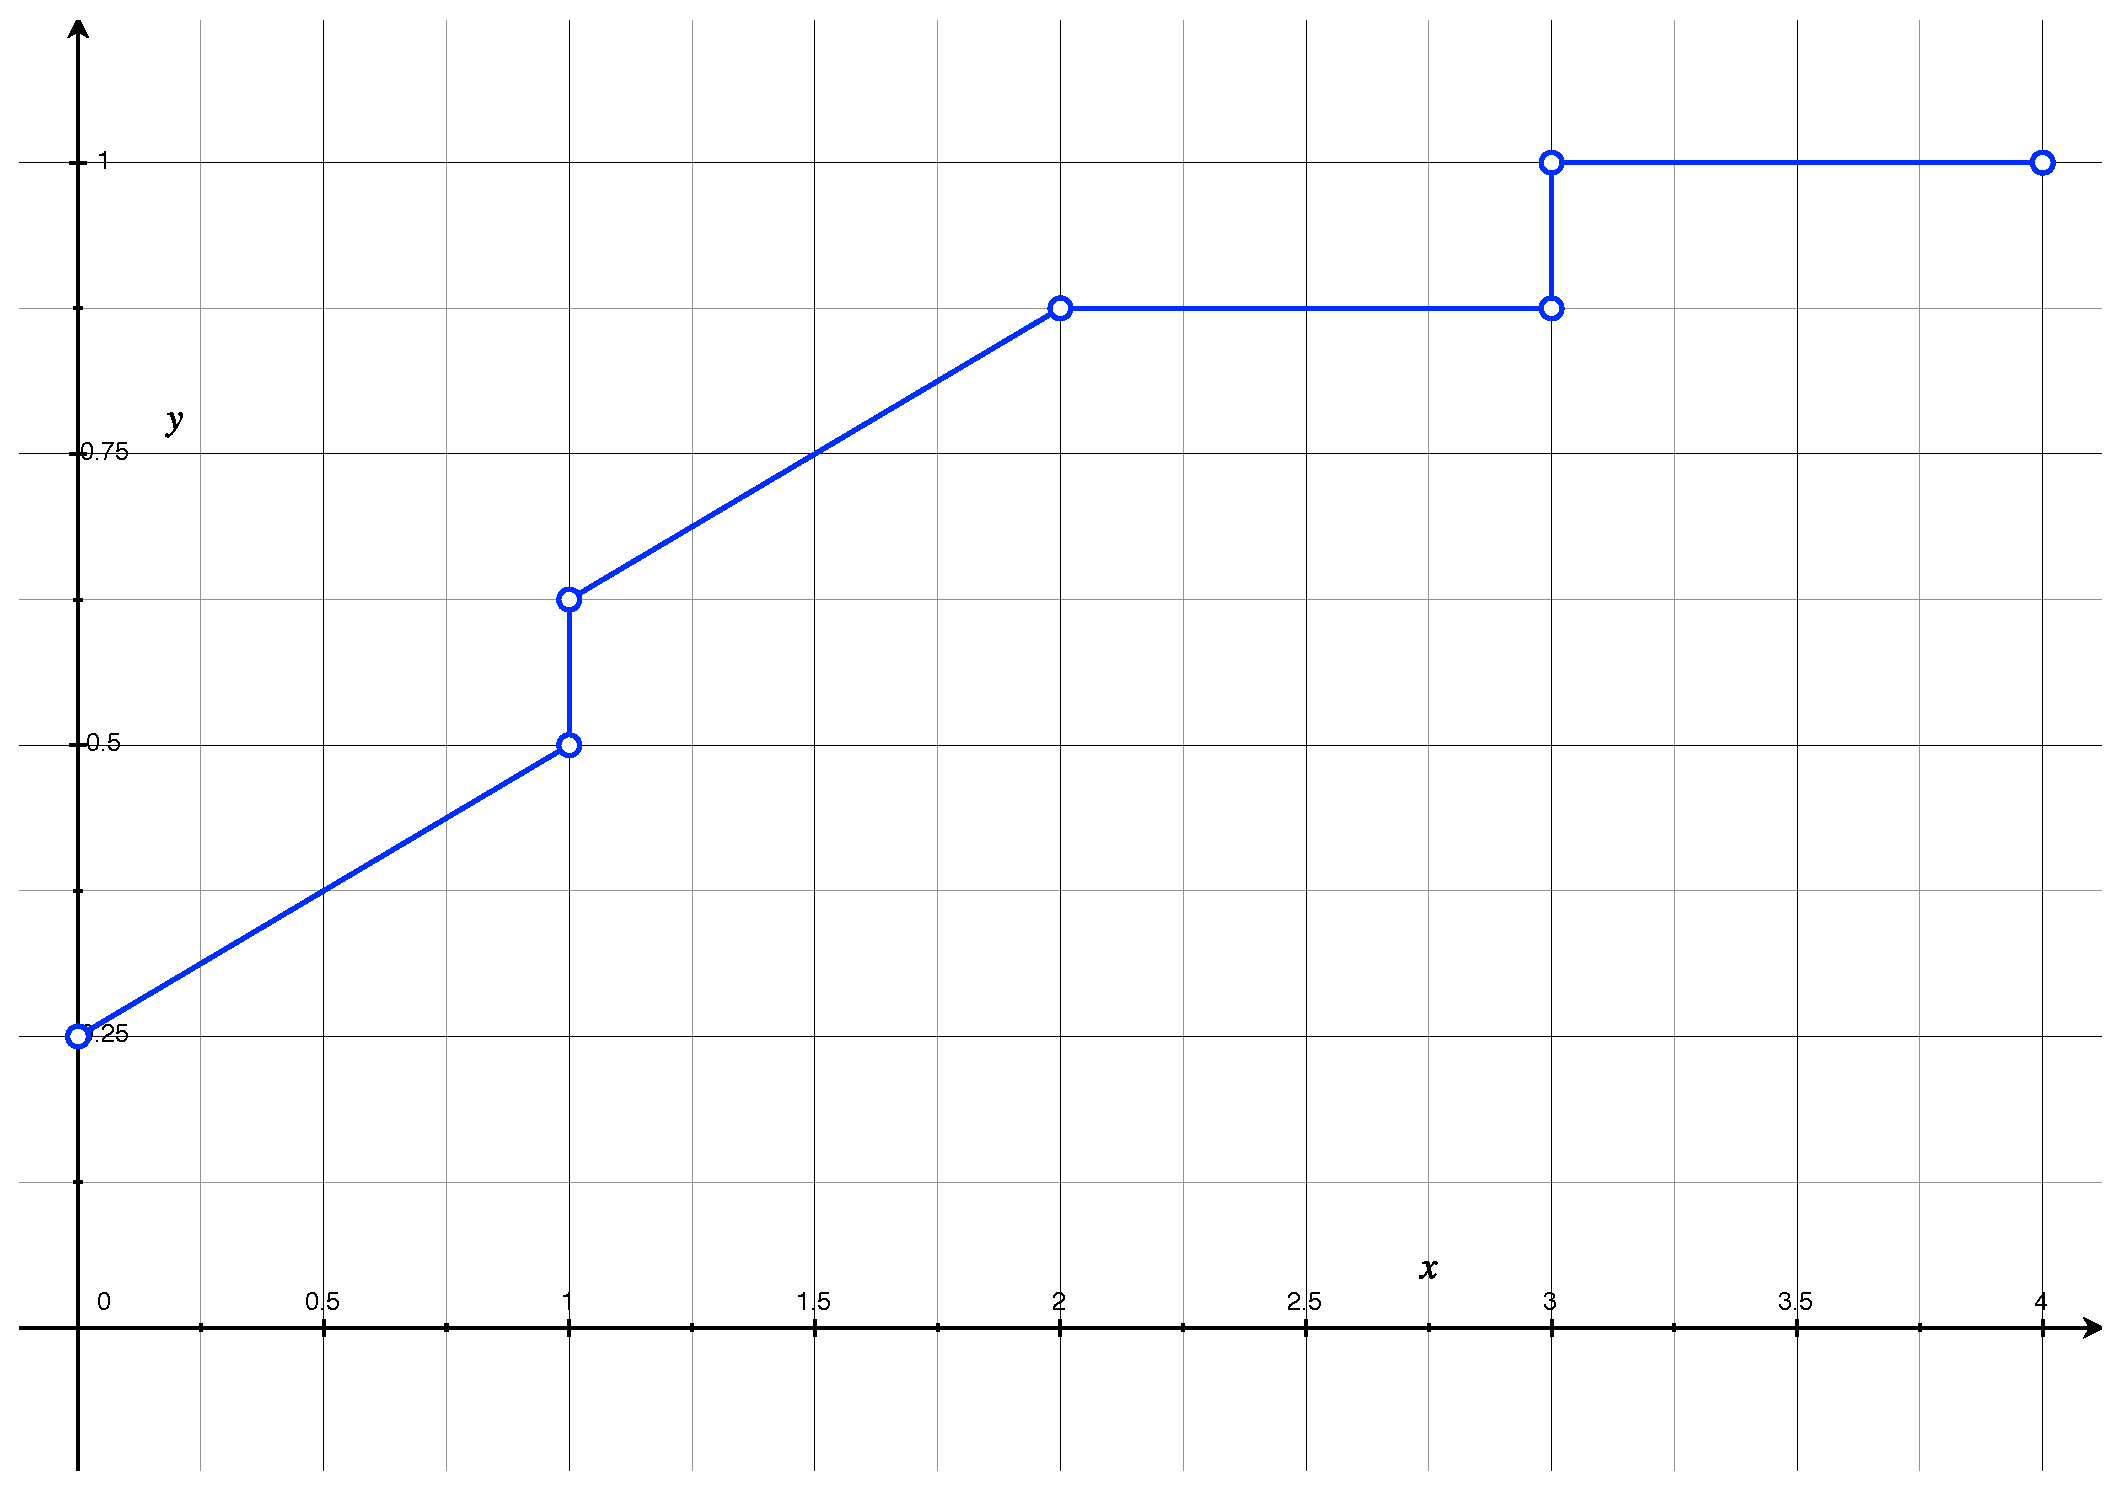
\includegraphics[width=0.48\textwidth]{6-fig}
      %   \end{center}
      %   \caption{$F_Z(z)$}
      %   \label{fig:6-fig}
      % \end{wrapfigure}
      \begin{figure}[ht]
        \centering
        \resizebox{.95\textwidth}{!}{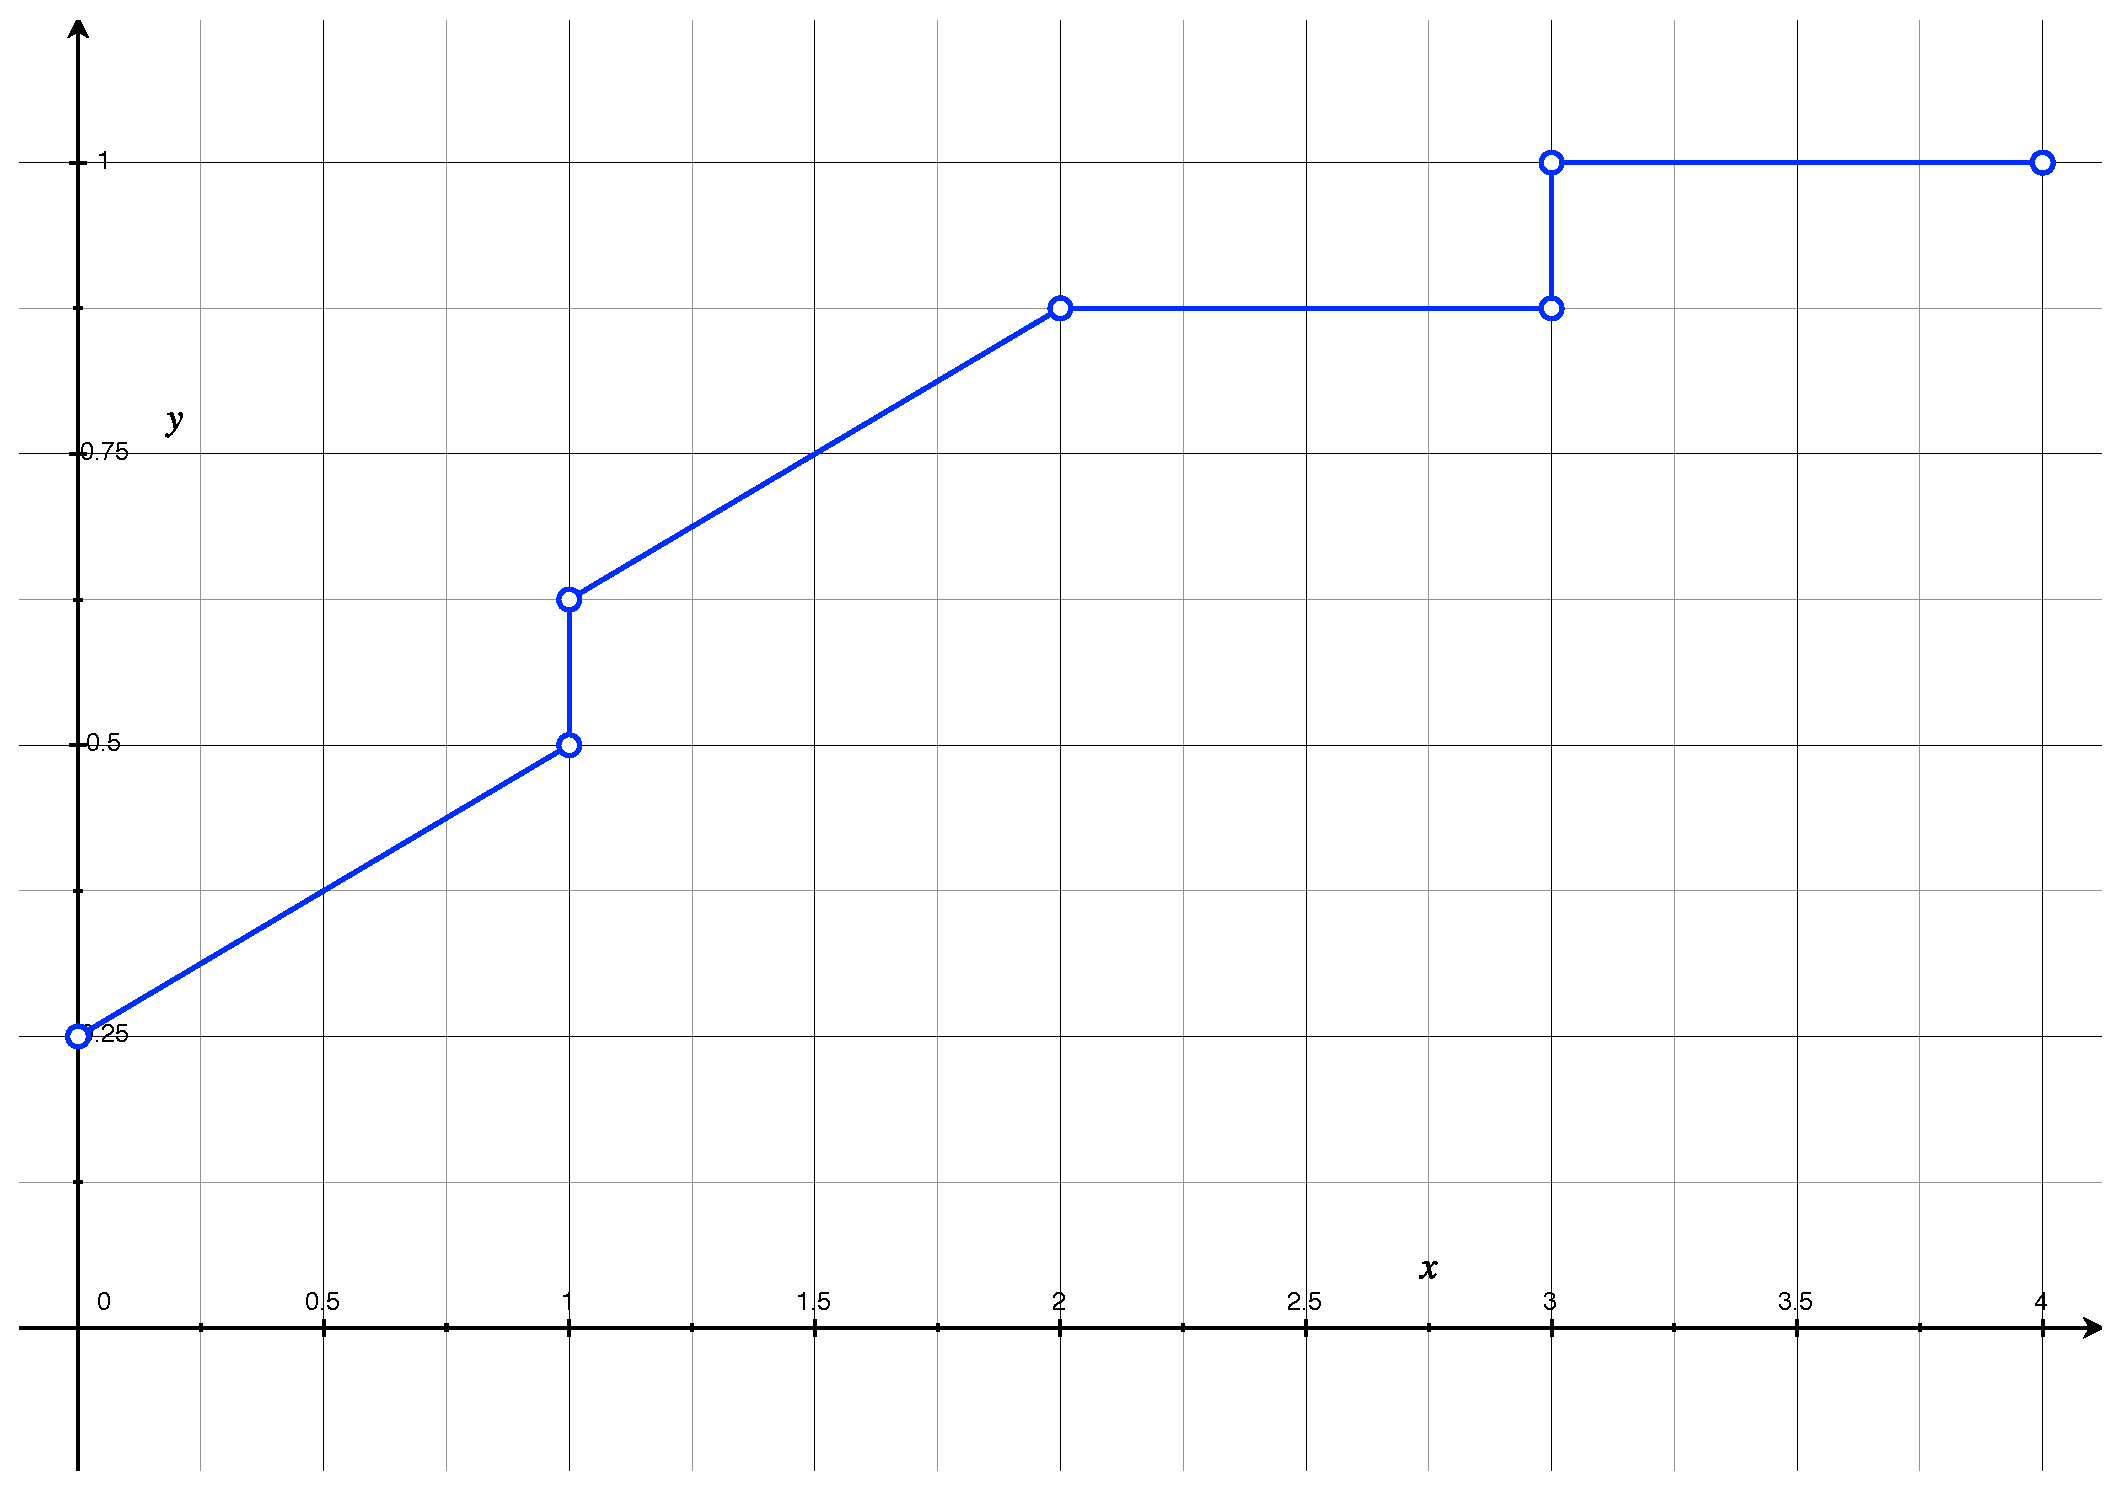
\includegraphics{6-fig}}
        \caption{$F_Z(z)$}
        \label{fig:6-fig}
      \end{figure}
    \end{enumerate}
    \begin{solution} \hfill \\\\ {\color{red} {\huge TODO}}
    \end{solution}
  \end{Ex}
\item
  \begin{Ex}
    Jane goes to the bank to make a withdrawal, and is equally likely
    to find 0 or 1 customers ahead of her. The service time of the
    customer ahead, if present, is exponentially distributed with
    parameter $\lambda$ What is the CDF of Jane's waiting time?
    \begin{solution} \hfill \\\\ {\color{red} {\huge TODO}}
    \end{solution}
  \end{Ex}
\end{enumerate}
\end{document}
